\section{Experiment 1: Horizontal and vertical bars}
\label{section:horvertAdaptiveInhibition}

\subsection{Introduction}

For this experiment the WTA network will be shown images of either horizontal or vertical bars. Through unsupervised learning the output neurons will learn to cluster the images together, depending on the orientation and position of the bars. 
The effect of the prior neurons will be demonstrated by generating ambiguous images which show a horizontal and a vertical bar at the same time. Depending on the activity of the prior neurons the output neurons will respond more to the horizontal, or to the vertical bar of the image. 

\subsection{Methods}

\paragraph{Input data}
Black bars with a width of seven pixels were drawn onto a white background with a size of 35 x 35 pixels. The bars could be oriented either horizontally or vertically. The network is supposed to cluster ten different groups within these images, five horizontally and five vertically. With a given bar width of seven pixels, and five groups in each direction the image height and width were determined as 35 pixels, to yield equally sized groups. The orientation of the training images was chosen randomly via a uniform distribution. The position of the bars in the images were uniformly distributed along the 35 pixels of either axis. To simulate noise each pixel of an image had a chance of ten percent to have its color flipped after the generation.
During the training of the network random images were generated and presented for 200 ms. As the simulation had a duration of 800 seconds this resulted in 4000 images shown to the network. Examples of the input data can be seen in Figure \ref{fig:horvertImages}. To show the value of the added a-priori information, validation images with two bars forming a cross were also generated, seen in Figure \ref{fig:horvertTrainingCrossImage}. When shown to the network in the validation process the prior neurons were given the information that a cross is either of horizontal or vertical orientation.

\begin{figure}
  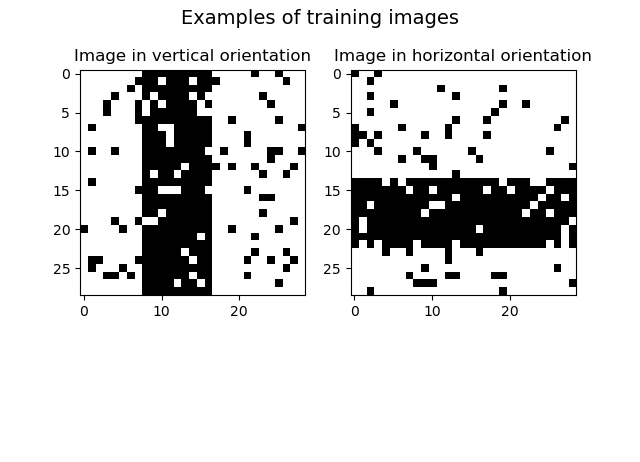
\includegraphics[width=\linewidth]{figures/horvert/horvertTrainingImages.png}
  \caption{Training images generated for experiment 1. One image of each possible orientation at a random position.}
  \label{fig:horvertImages}
\end{figure}

\begin{figure}
\centering
  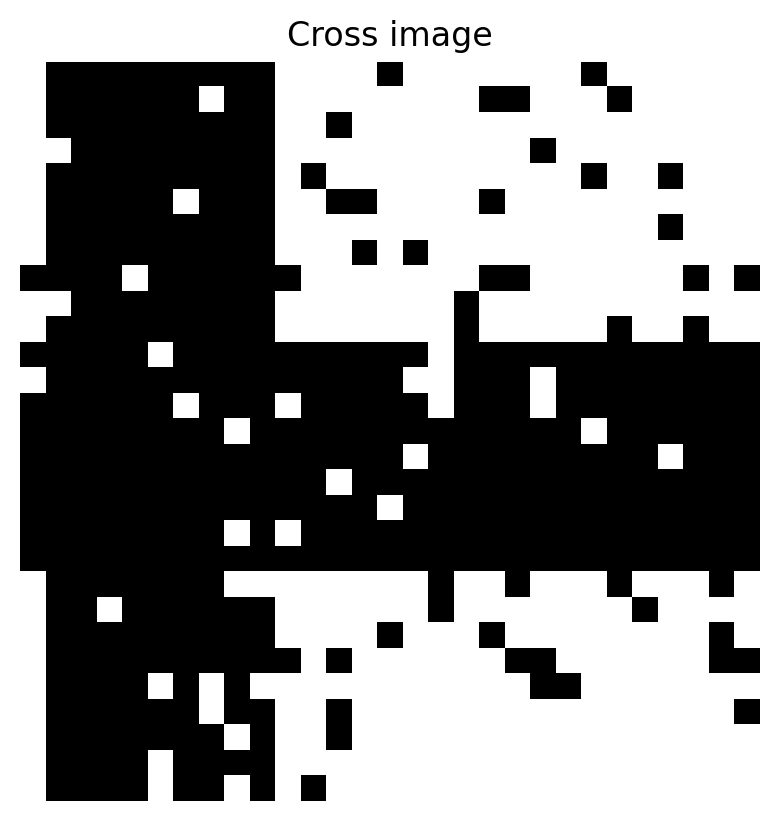
\includegraphics[width=0.6\linewidth]{figures/horvert/horvertTrainingCrossImage.png}
  \caption{Generated cross image which can represent either horizontal or vertical orientation.}
  \label{fig:horvertTrainingCrossImage}
\end{figure}

\paragraph{Network architecture}

As every pixel of the shown images was connected to two input neurons the network had 1682 input neurons. Each of these neurons had a firing frequency of 20 Hz, when in the active state. Then there were ten output neurons, one for each possible group. Lastly, there were two equal sized groups of prior neurons. During training the first group $z^h$ was active when the image was of horizontal orientation and the other group $z^v$ was active for vertical orientation. The number of prior neurons and their firing frequency had to be determined via grid search, as they needed to be set at values where the impact of the a-priori information is neither to strong nor to weak.

\paragraph{Network and simulation parameters}

The simulation of the experiment was performed in time steps of 1 ms. This step size was used for all experiments. As given by \citet{nessler} the time window $\sigma$ was 10 ms, the time constant for the rise of the EPSPs $\tau_{rise}$ was 1 ms and the time constant for the decay of the EPSPs $\tau_{decay}$ was 15 ms. Before performing this experiment, Experiment 2 of \citet{nessler} was reproduced to validate that the implementation of the simulation was correct. This proof of concept was omitted in this work, however within it the weight shift parameter $c = 20$ and the learning rate $\lambda = 10^-3$ were determined via grid search. These parameter values were reused for this experiment, as the input data, as well as the network architecture, were similar.

\subsection{Results}

%TODO check ALL plots EVERYWHERE for correct weight nomenclature

First different numbers of prior neurons were tried. Simulations with 10, 20, 50, 100 and 200 prior neurons were performed. For 50, 100 and 200 prior neurons the training process was impaired by the activity of the prior neurons. Some output neurons were responding to too large areas, while other prior neurons were not responding to any specific areas at all. With a number of 10 and 20 prior neurons each of the prior neurons learned to respond to either horizontal or vertical images. To maximize the impact of the a-priori information the validation of the network was performed with 20 prior neurons, as it was the largest number that resulted in a properly trained network. The results of the training process can be seen in Figures \ref{fig:horvertAdaptiveInhibitionTraining} and
%TODO above... horvertAdaptiveInhibitionTraining auch gleiche Qualität bringen wie die validation plots :/
 \ref{fig:horvertAdaptiveInhibitionpriorWeights}.
%TODO above... horvertAdaptiveInhibitionpriorWeights think if I want to leave this in and mby improve plot
%1. color code instead of black white
%2. check and fix subplot titles
%3. ylabel


\begin{figure}
  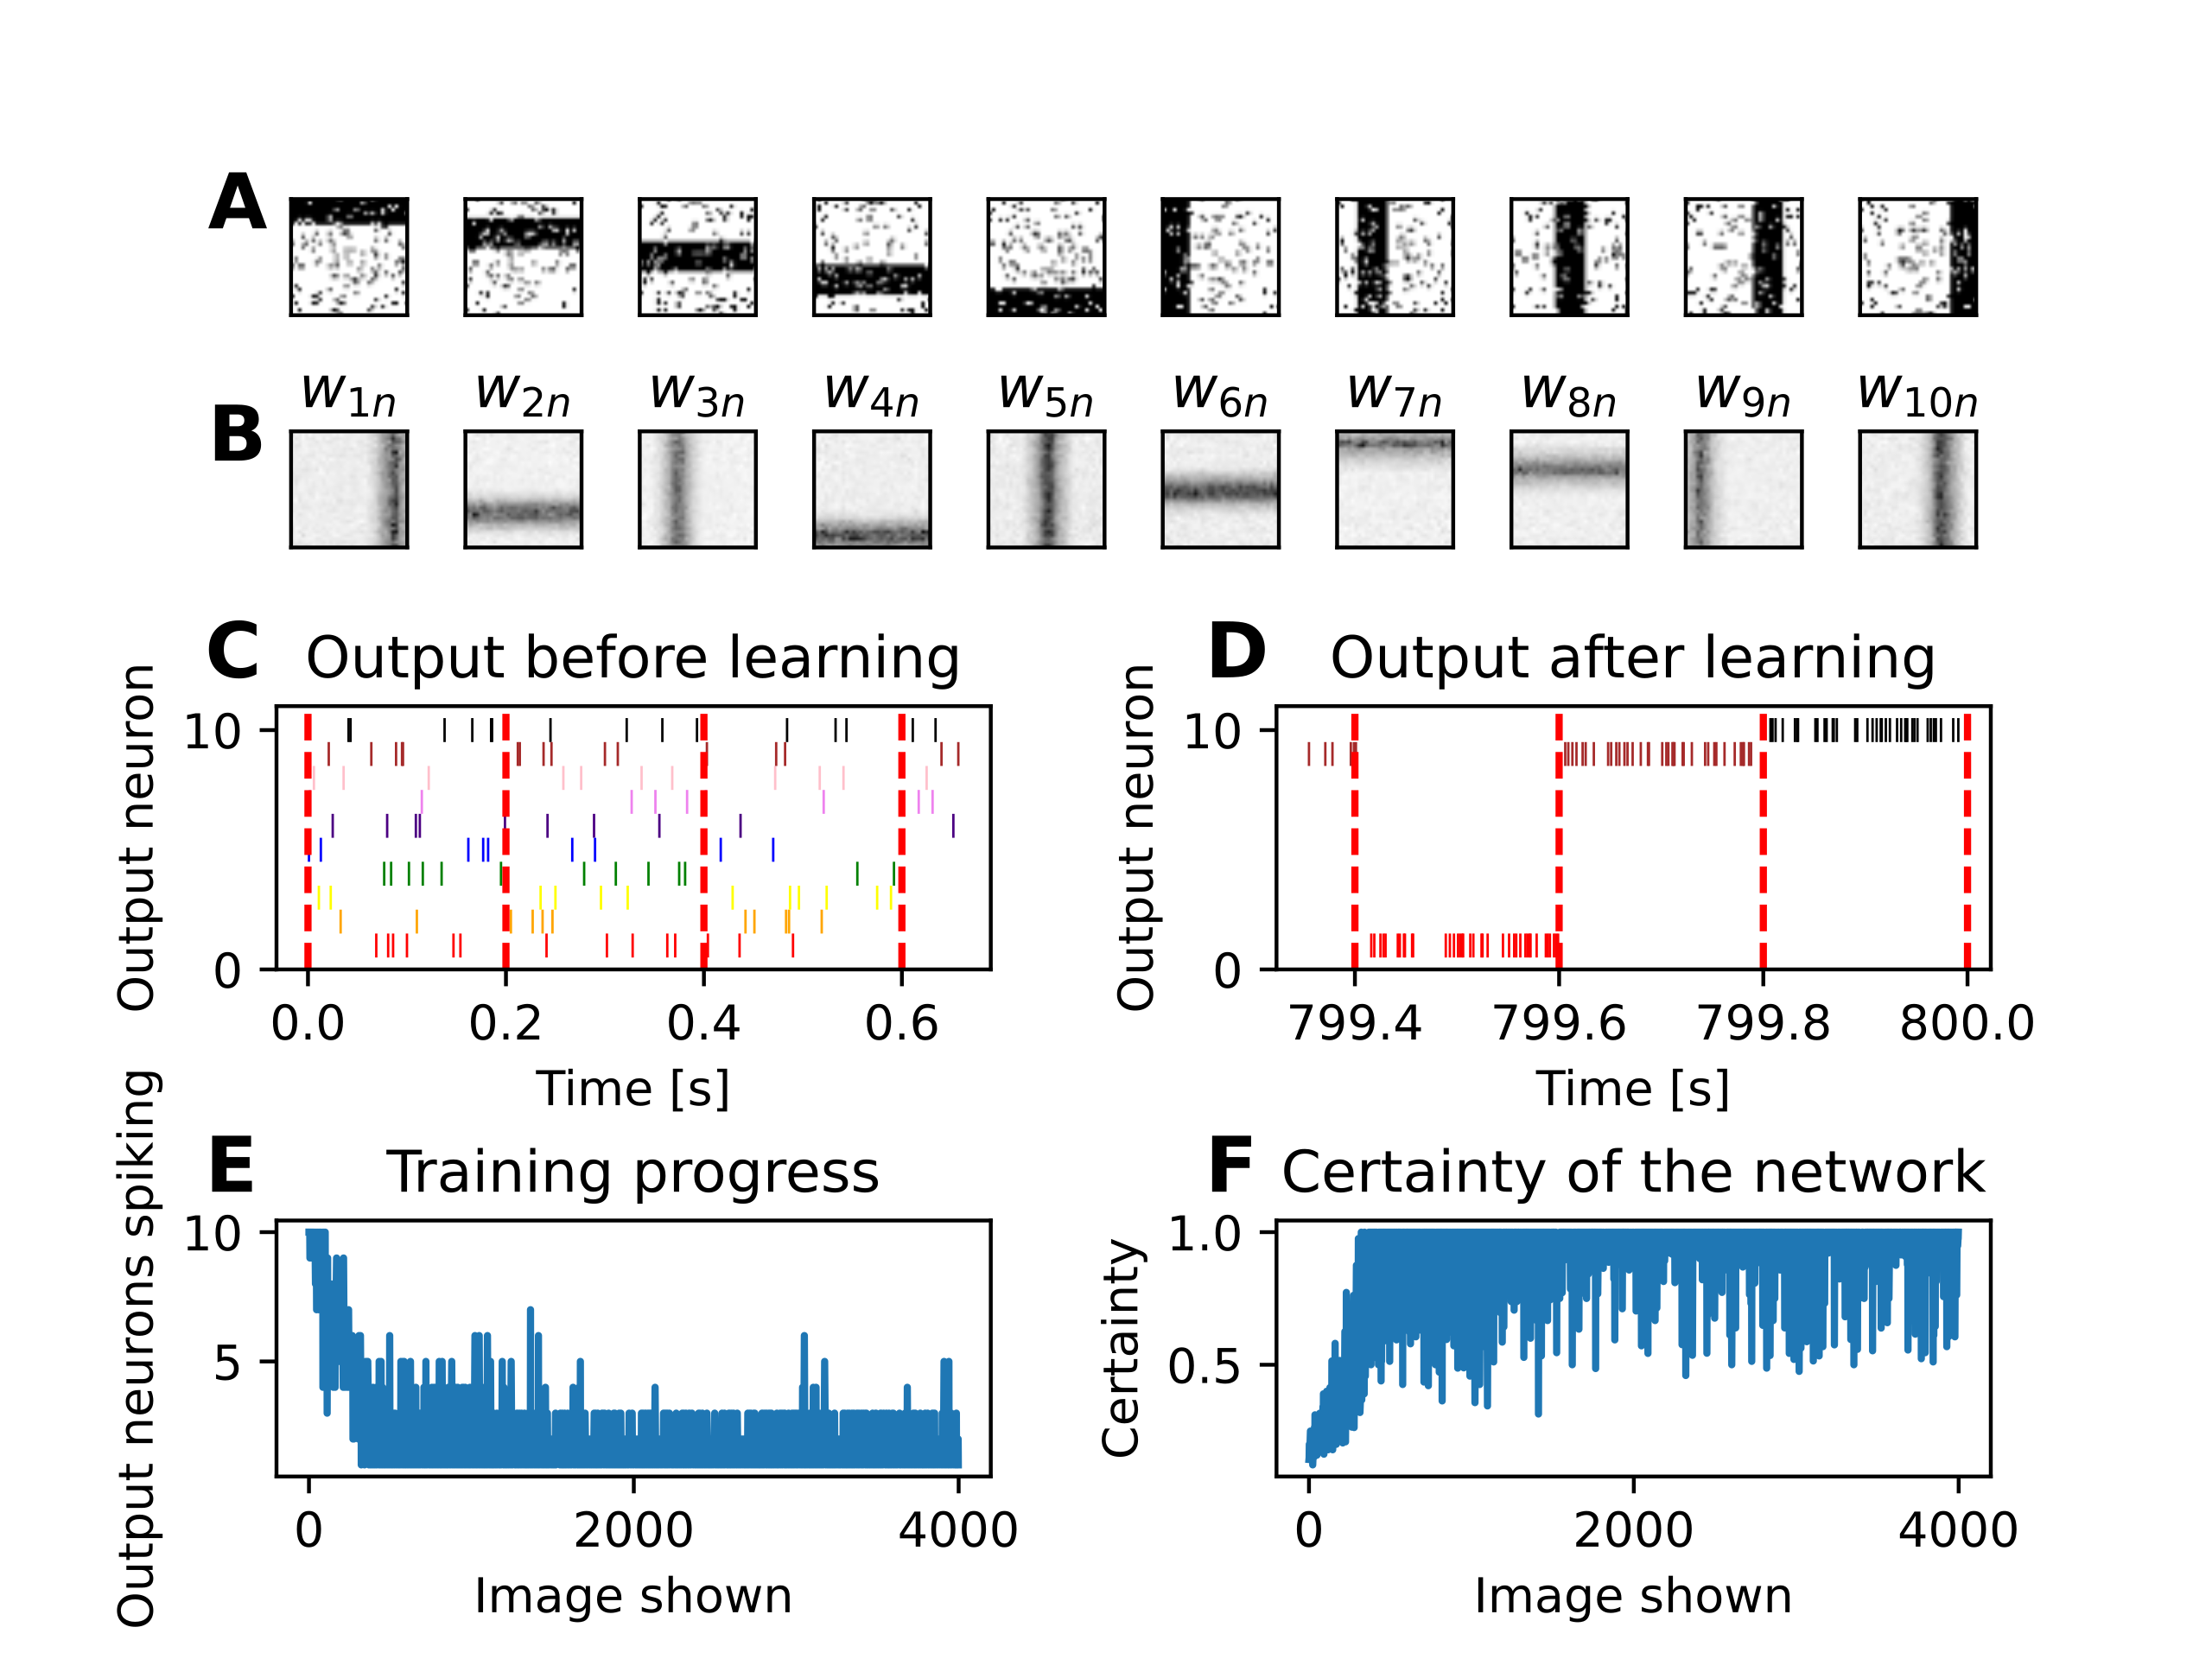
\includegraphics[width=\linewidth]{figures/horvertAdaptiveInh/trainingPlot.png}
  \caption{\textbf{Training with 20 prior neurons.} \textbf{A} Examples of 35 x 35-pixel input images of horizontal and vertical bars with background noise. \textbf{B} Learned weights of the connections between input and output neurons. \textbf{C, D} Spike activity expressed by the output neurons before and after the training of the network. \textbf{E} Number of distinct output neurons active during the presentation duration of each training image. \textbf{F} Number of spikes of the most active output neuron divided by the number of spikes of all other output neurons during the presentation duration of every training image.}
  \label{fig:horvertAdaptiveInhibitionTraining}
\end{figure}

\begin{figure}
  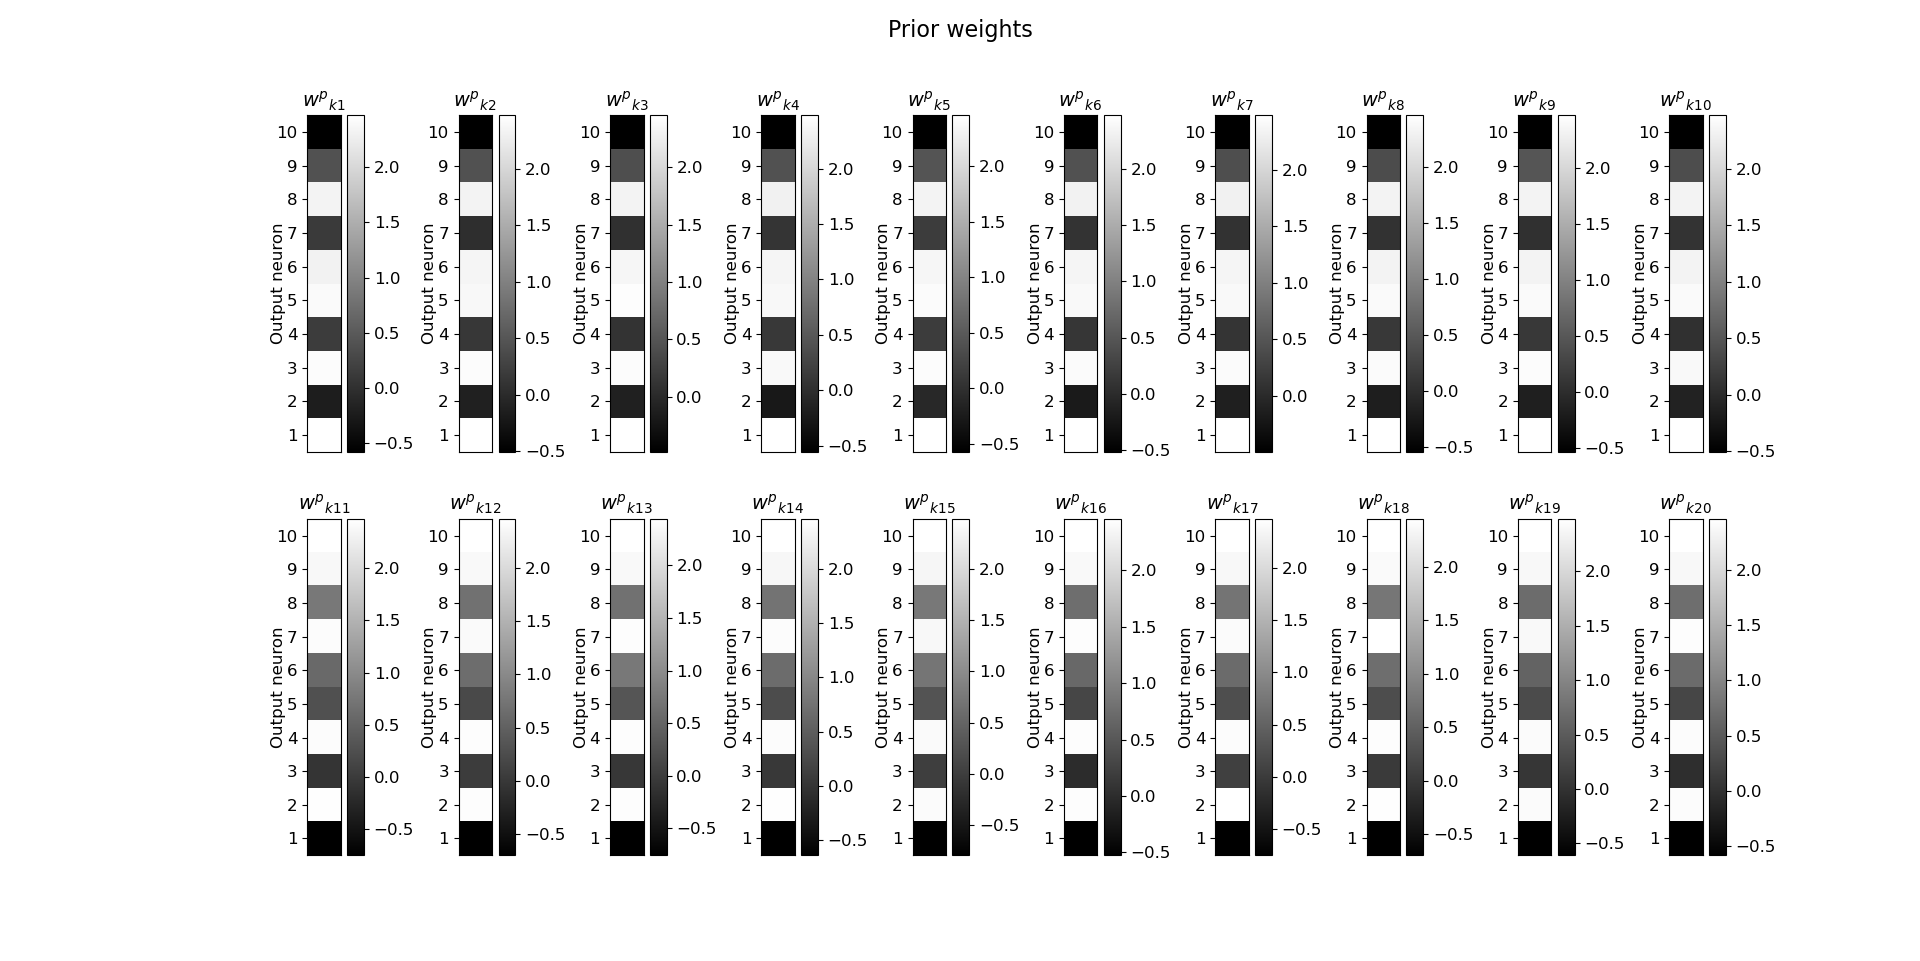
\includegraphics[width=\linewidth]{figures/horvertAdaptiveInh/priorWeights.png}
  \caption{ Learned weights of the connections between prior and output neurons. }
  \label{fig:horvertAdaptiveInhibitionpriorWeights}
\end{figure}

%TODO add the horizontal and vertical validation!

To validate the learning outcome of the training the network was shown horizontal bars at every possible position in the image for 200 ms each and the output neuron activity was recorded. To visualize which output neuron is the most active for each position a horizontal bar with a height was drawn into a 35 x 35 pixel image, color-coded to represent the respective output neuron. This can be seen in Figure  TODO


%TODO update description, as image was updated
\begin{figure}
  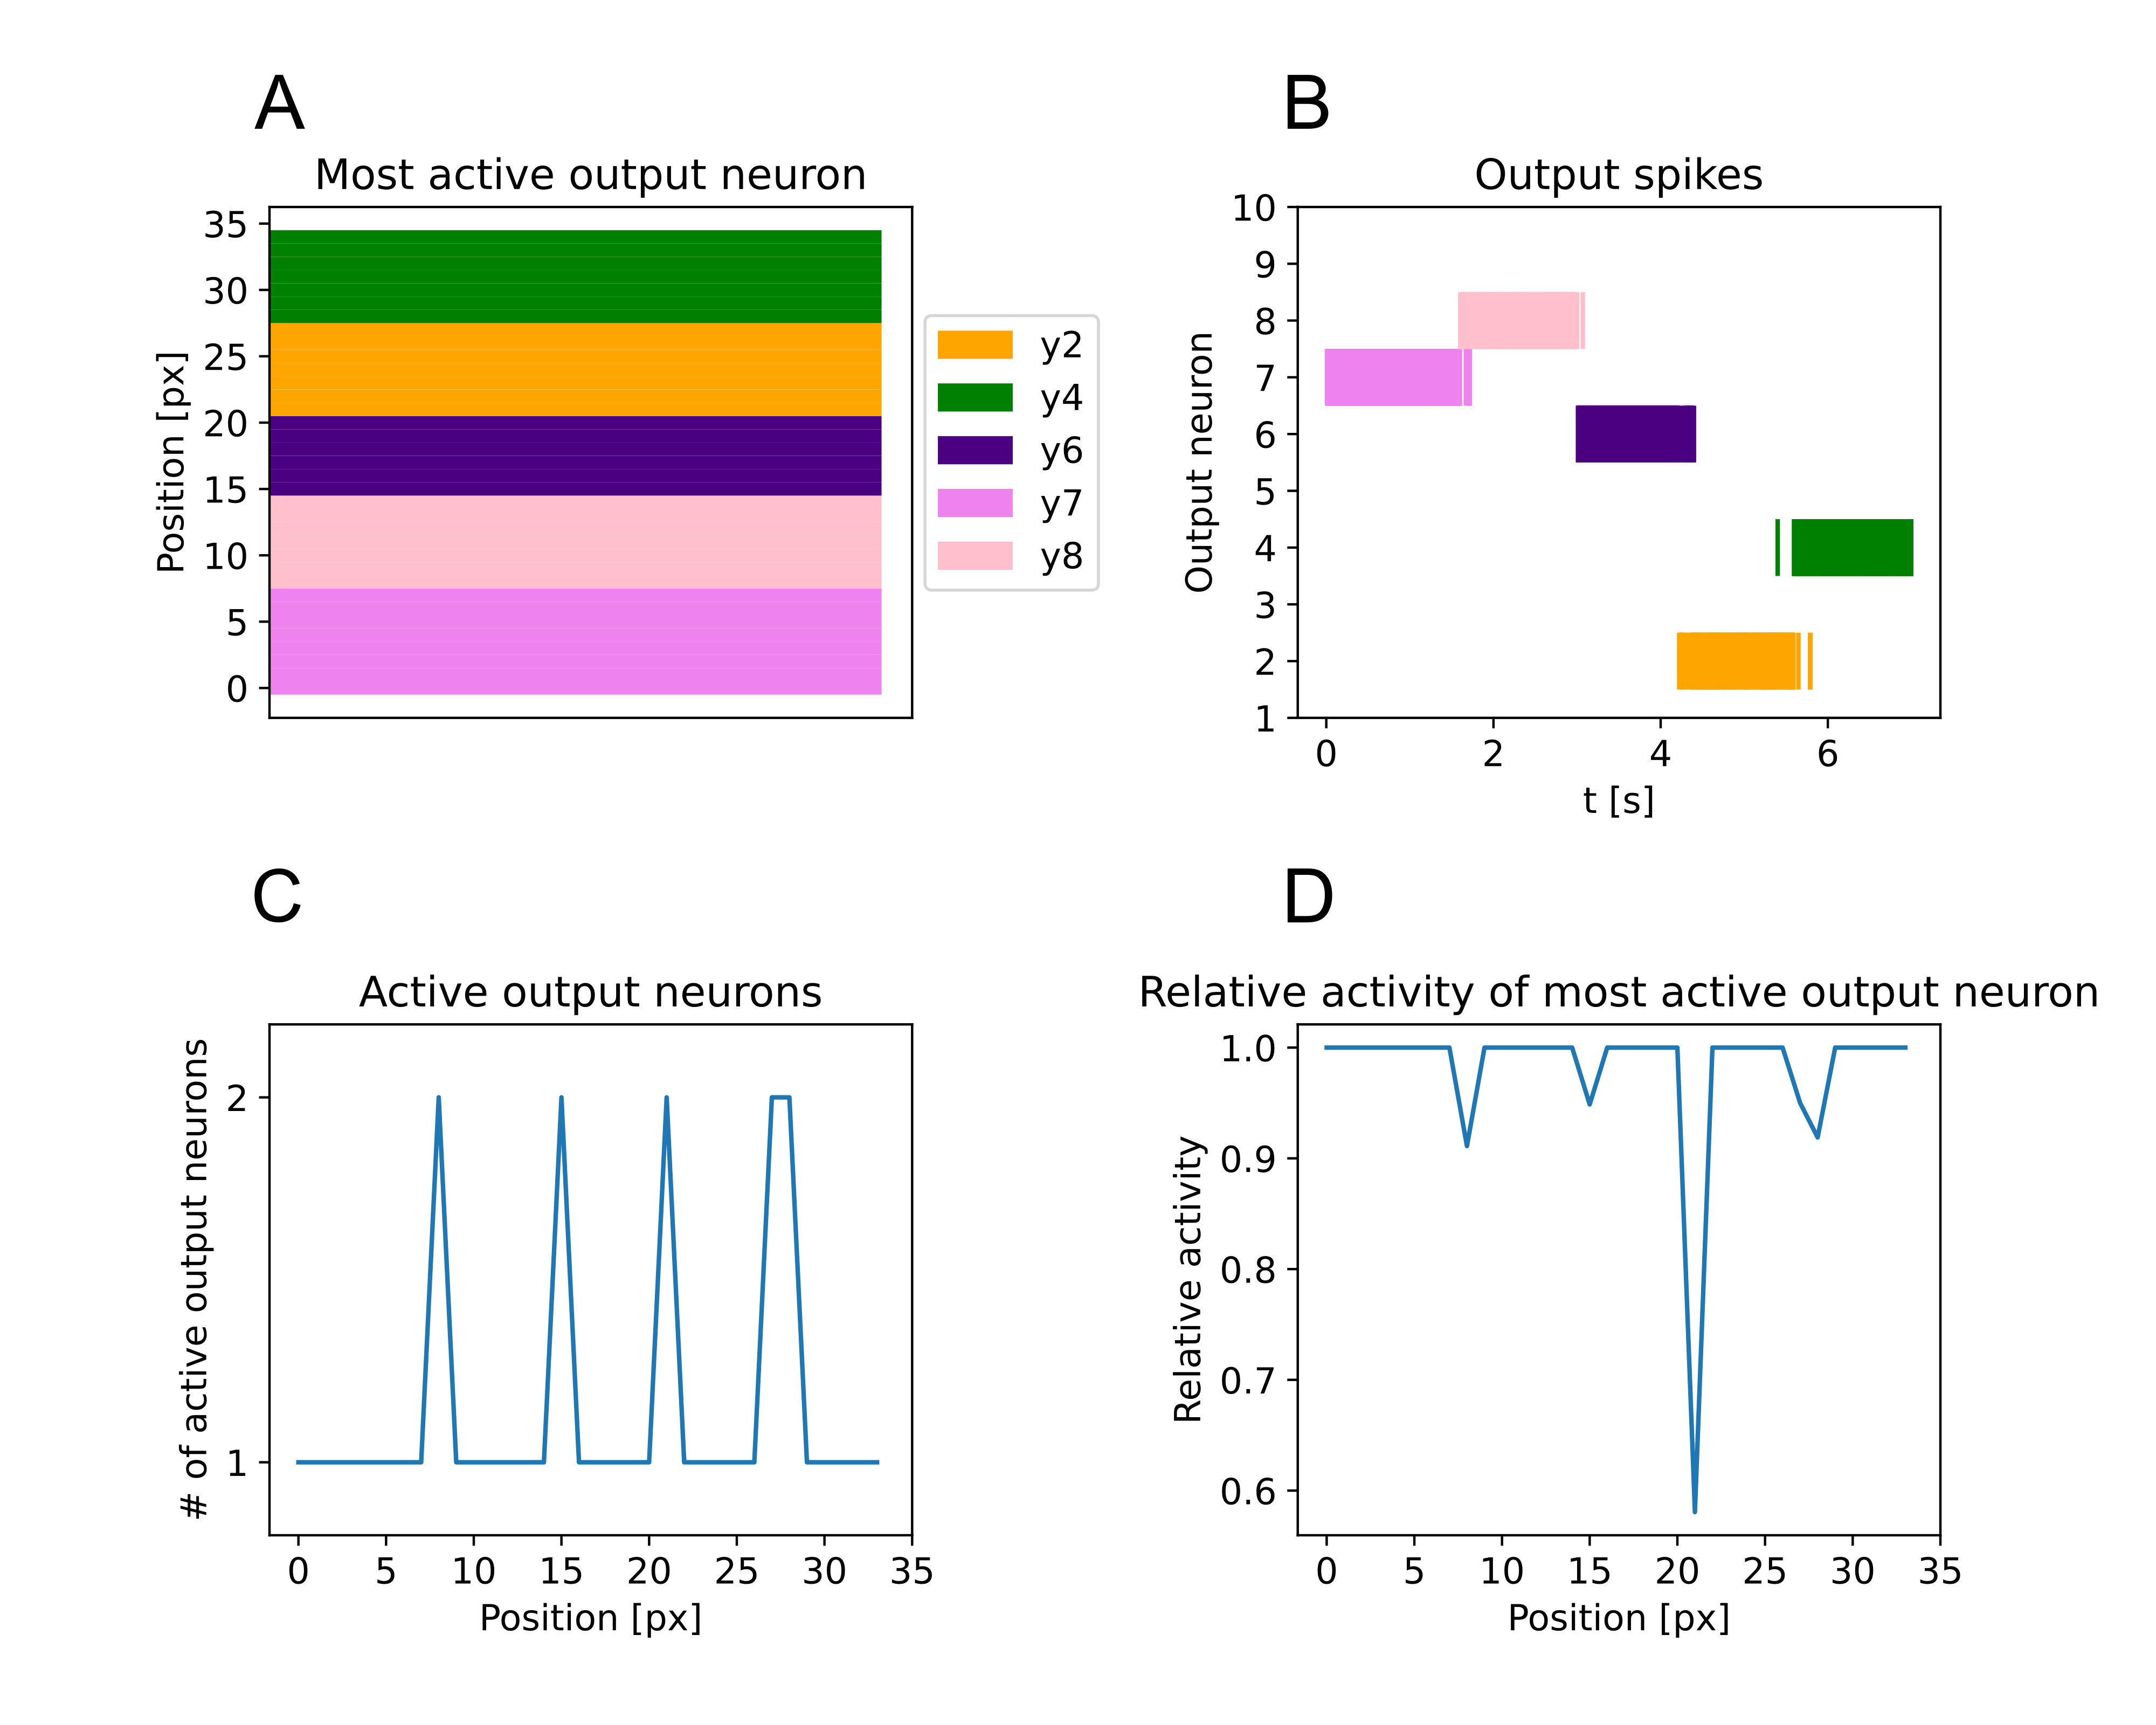
\includegraphics[width=\linewidth]{figures/horvertAdaptiveInh/horizontal_validation.png}
  \caption{\textbf{Horizontal validation.} \textbf{A} Most active output neuron, depending on the vertical position of a horizontal bar.  \textbf{B} Output spikes during the validation process. \textbf{C} The number of distinct output neurons spiking depending on the vertical position of a horizontal bar.  \textbf{D}  }
  \label{fig:horvertAdaptiveInhibitionHorizontalValResults}
\end{figure}

%TODO same for vertical
 The vertical was done analogously
 
Every one of the ten output neurons responds primarily to one coherent area in one orientation.
During the validation of all possible horizontal bar images the output spike activity was recorded and how many distinct output neurons were spiking during each image presentation period. For the parts where the 7 pixels high bar in the image did not overlap the areas of two output neurons only one output neuron was active. Only in the border areas there were two output neurons active. This can be seen in Figures \ref{fig:horvert_c20_3_Zfactor5_horizontalDistinctZ} and \ref{fig:horvert_c20_3_Zfactor5_horizontalZSpikes}.





Next the impact of the prior was analysed. To do this an image with a horizontal (at pixel 12) and a vertical bar (at pixel 5) on it was generated. Then the prior was once set once to horizontal and once to vertical. The image and the prior was then fed to the network. The results can be seen in Figure \ref{fig:horvertAdaptiveInhibitionPriorValResults}.

\begin{figure}
  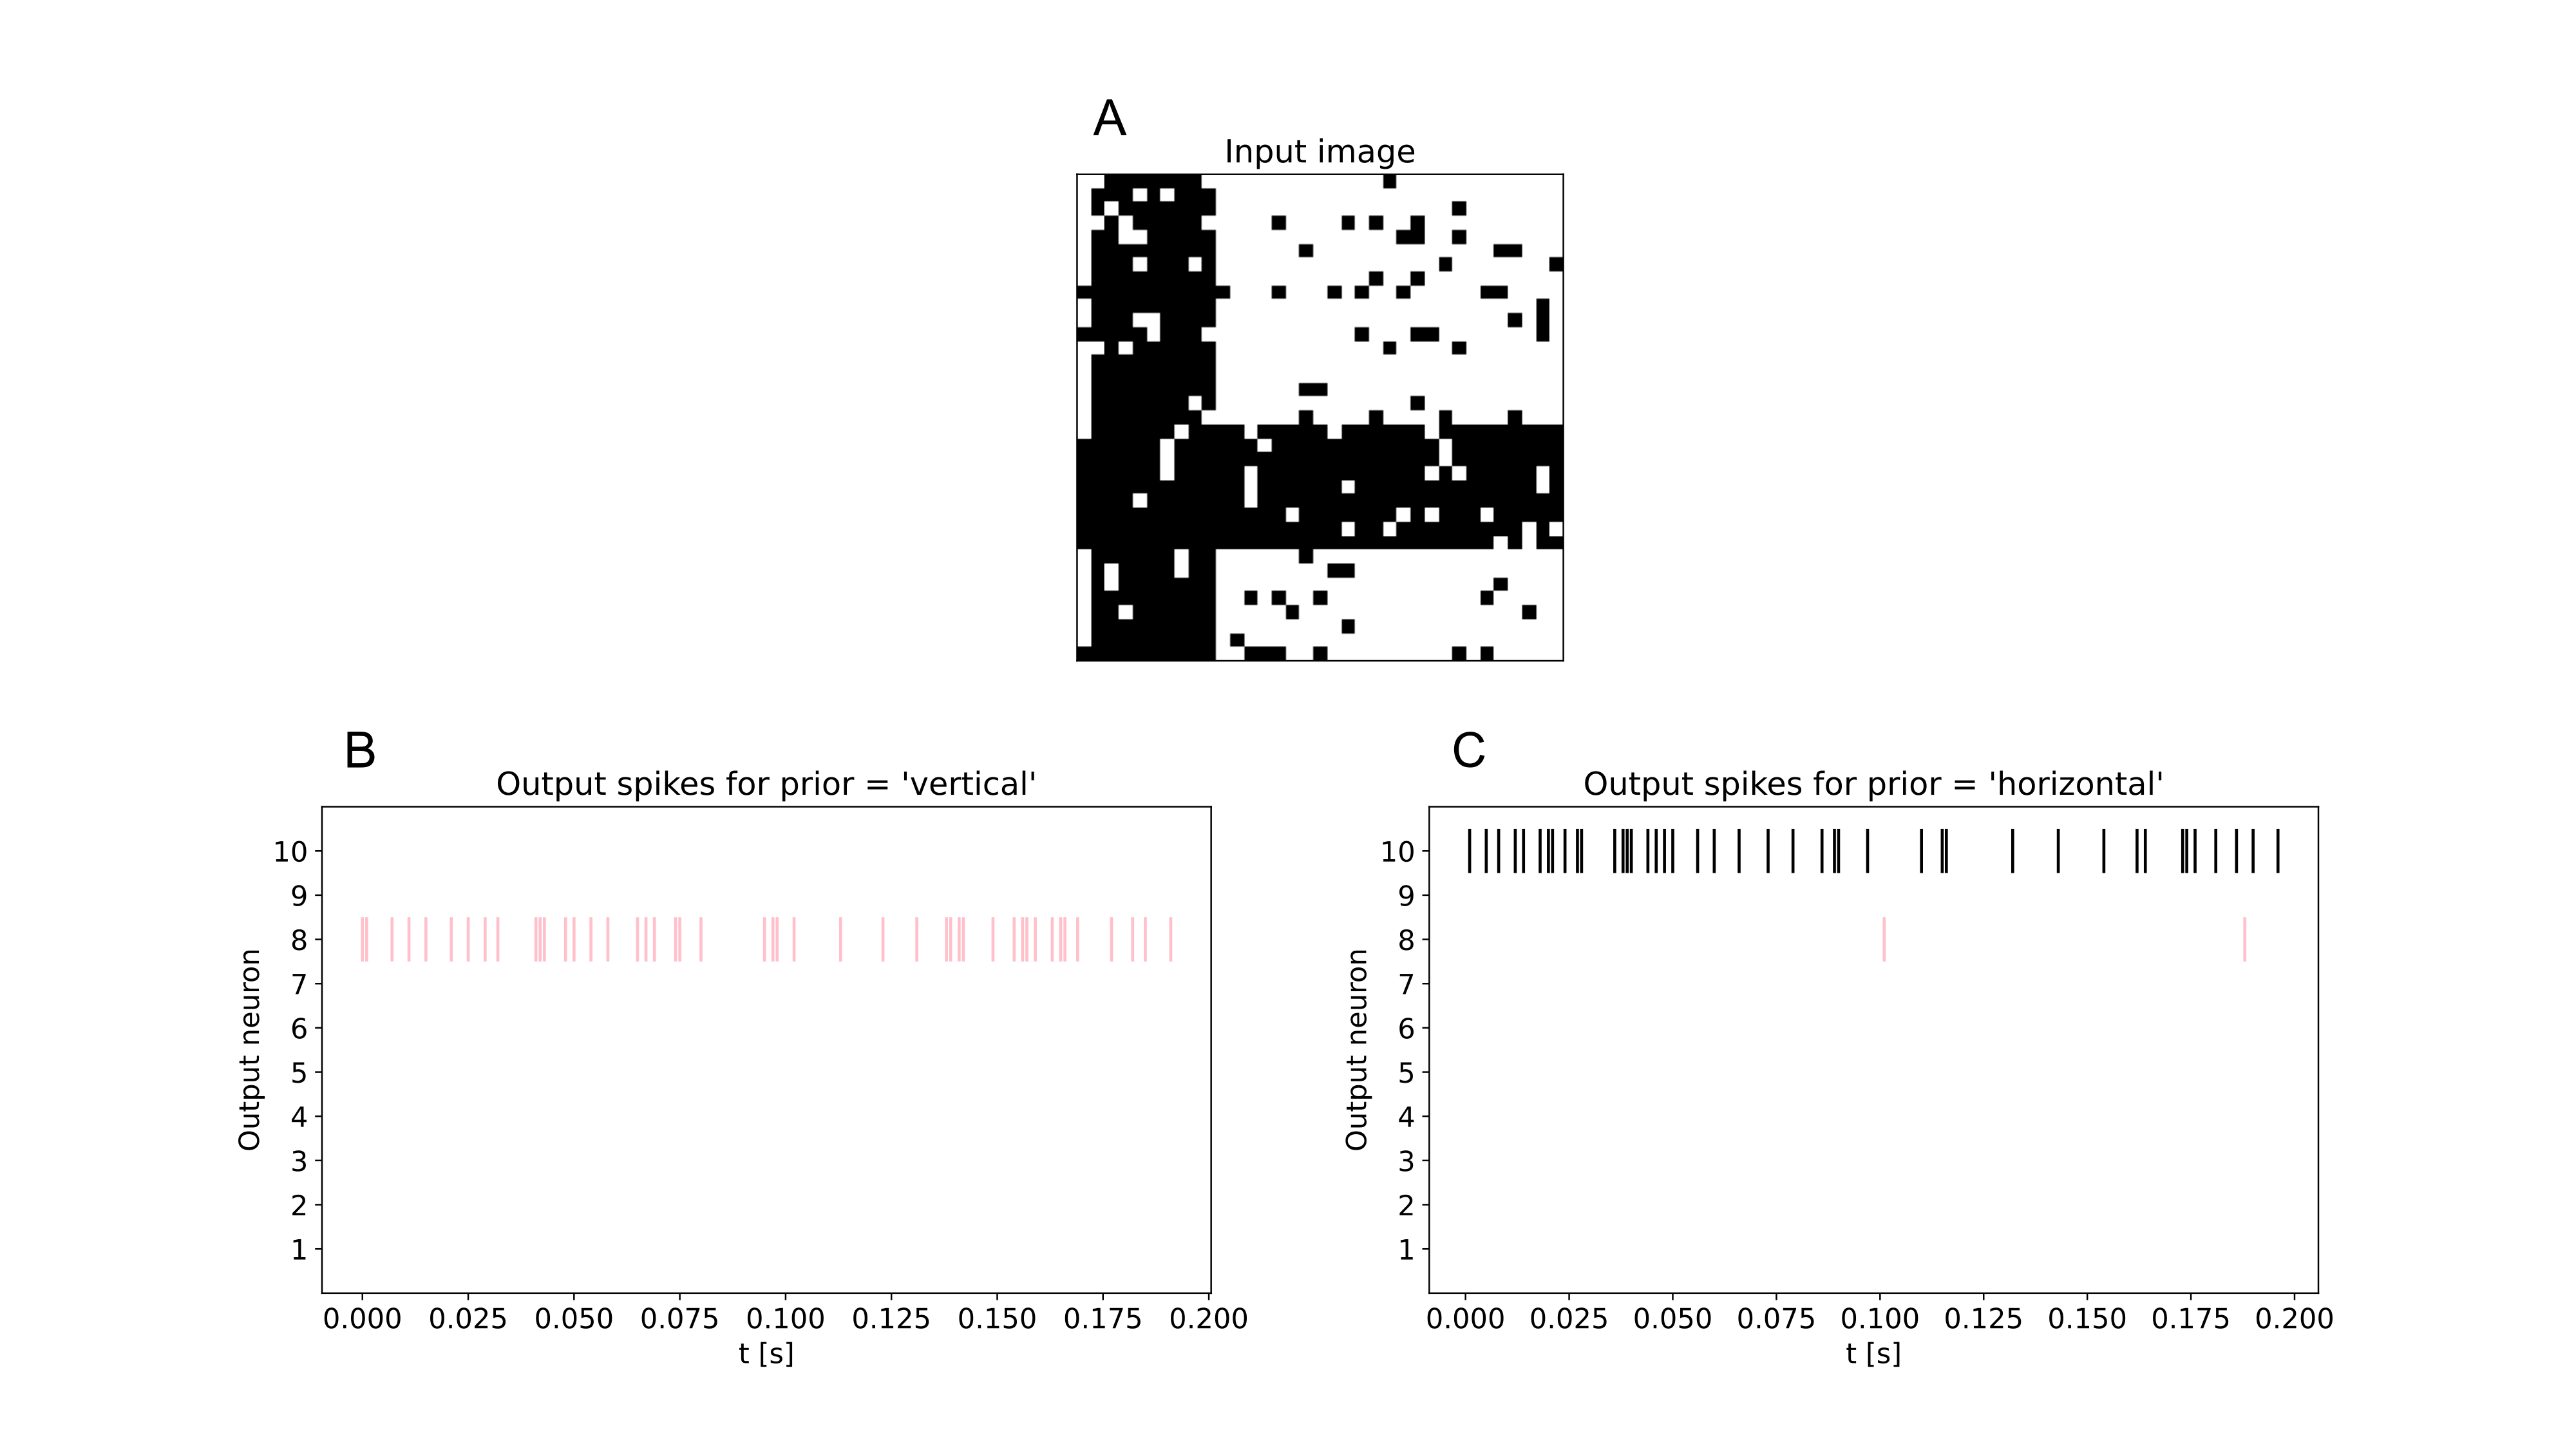
\includegraphics[width=\linewidth]{figures/horvertAdaptiveInh/20priors_pos5and12/crossValidation.png}
  \caption{\textbf{Impact of the prior Neurons.} \textbf{A} Image with a horizontal and a vertical bar on it that was fed to the network. \textbf{B} Spiking activity of the output neurons with prior = 'horizontal'. \textbf{C} Spiking activity of the output neurons with prior = 'vertical'. }
  \label{fig:horvertAdaptiveInhibitionPriorValResults}
\end{figure}

To better show the impact of the prior, the firing frequencies of the prior neurons were gradually changed. The starting firing frequency of $z^h$ was 200 Hz and 0 Hz for $z^v$. For those firing frequencies a cross image was shown to the network for 200 ms. After each image presentation duration the firing frequency of $z^h$ was decreased by 1 Hz and increased by 1 Hz for $z^v$. The used cross image can be seen in Figure \ref{fig:horvertAdaptiveInhibitionVariablePriorResults} A. The firing frequency of the 2 most active output neurons depending on the firing frequency of $z^v$ can be seen in Figure \ref{fig:horvertAdaptiveInhibitionVariablePriorResults} B. At the beginning $y_2$, which represents the horizontal part of the cross image, was the most active neuron, which is correct as the prior neurons fully supported a horizontal orientation of the input image. With rising firing frequency of $z^v$ the activity of the $y_2$ decreased and the activity of $y_8$ increased. This happened because the prior neurons gradually supported the interpretation of the image as vertical more and more.

\begin{figure}
  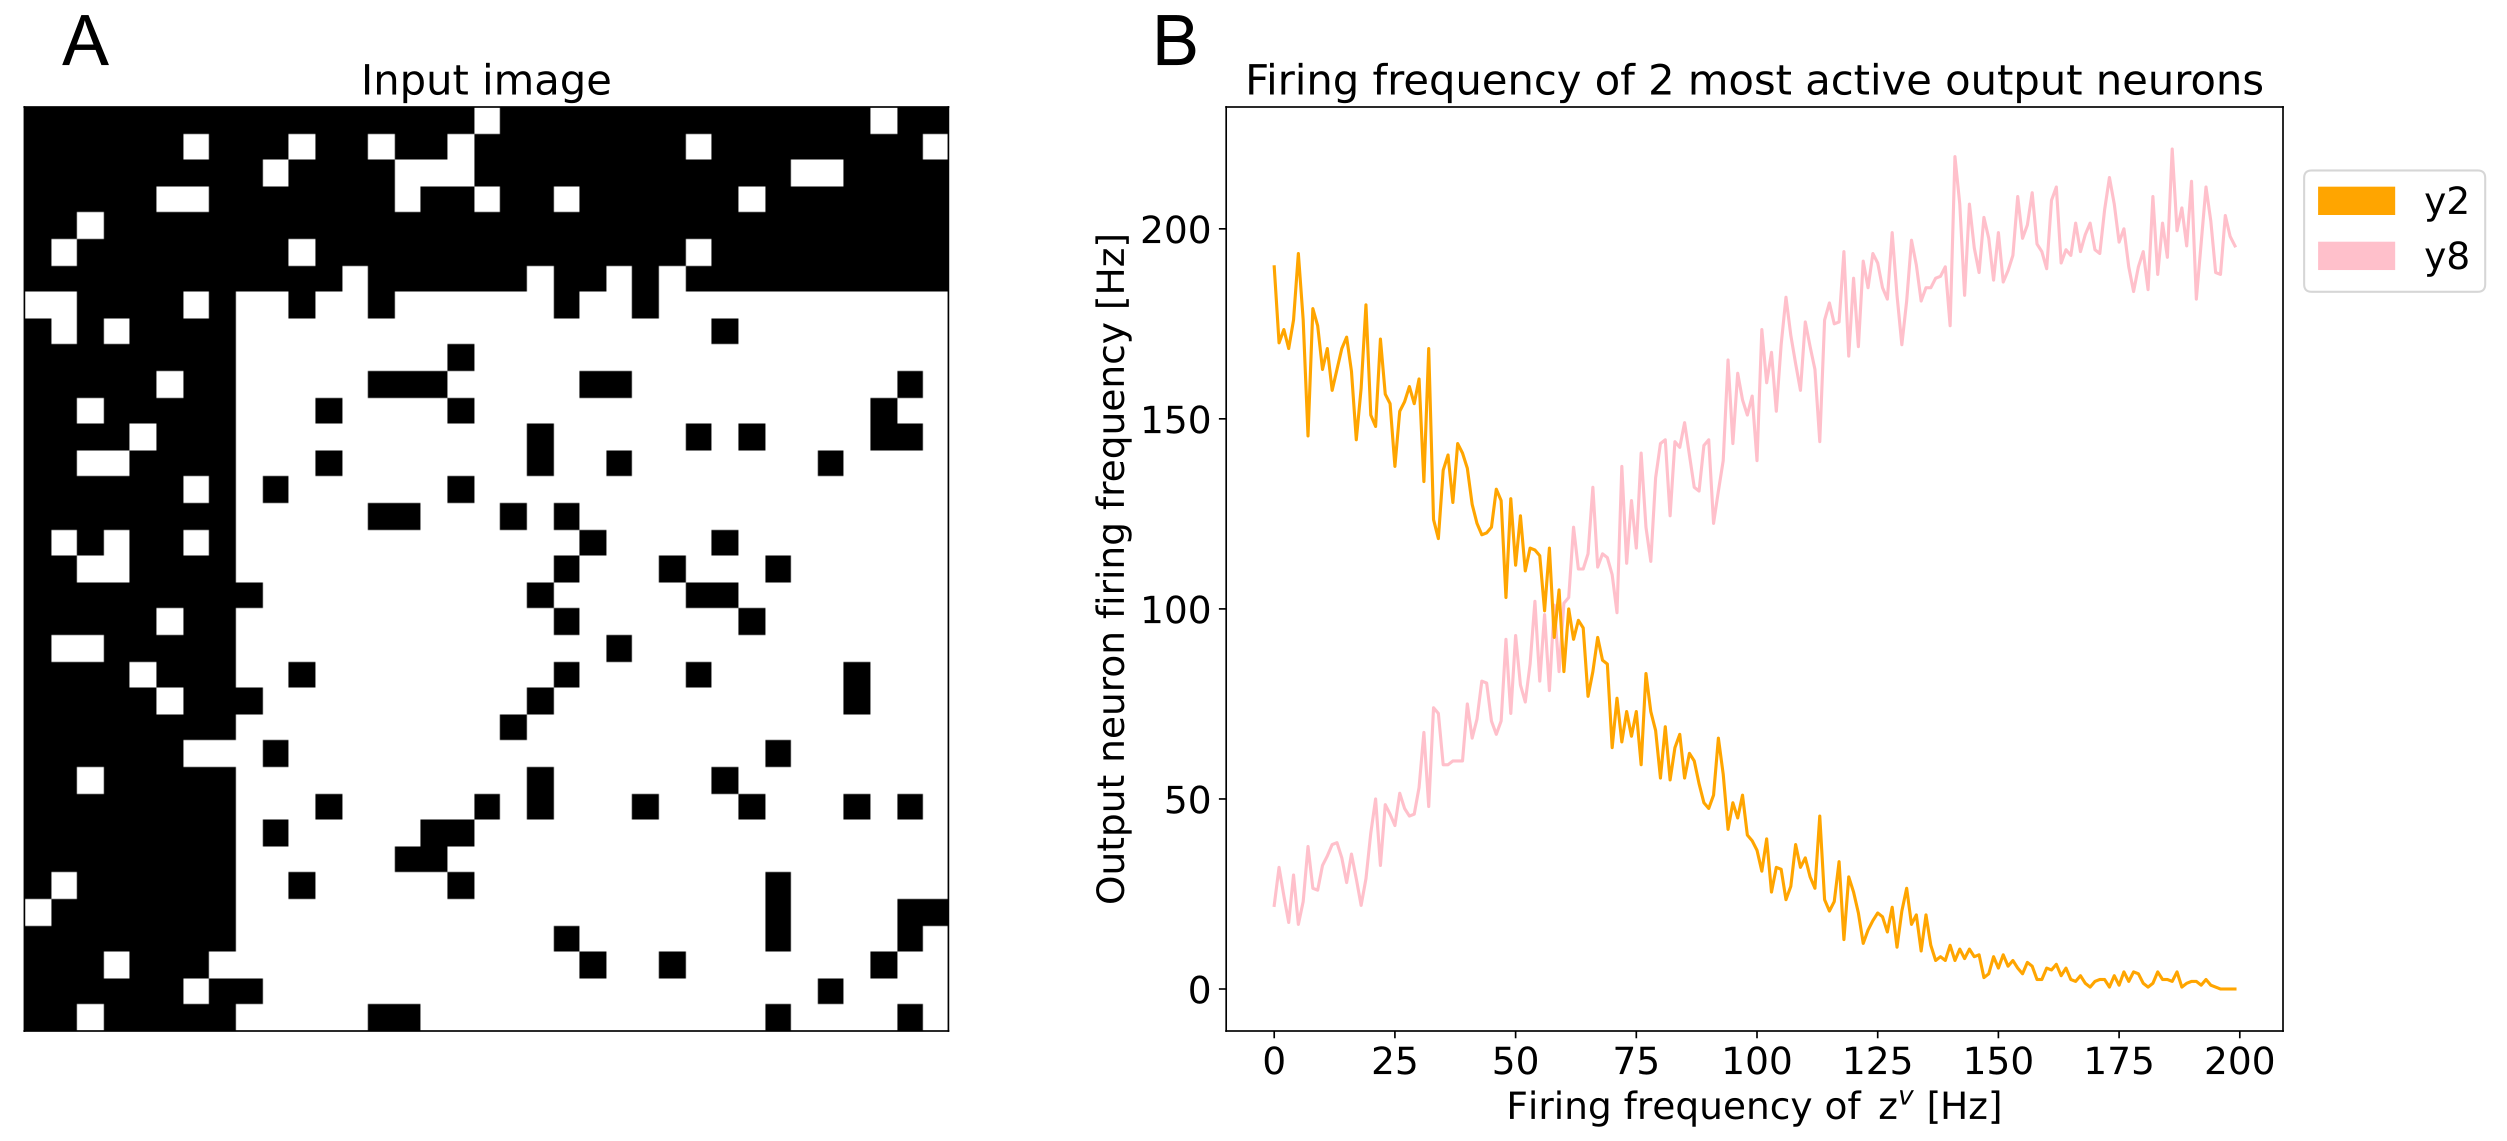
\includegraphics[width=\linewidth]{figures/horvertAdaptiveInh/YFrequency_prior.png}
  \caption{\textbf{Cross image with varying prior neuron activity.} \textbf{A} Cross image fed to the network. \textbf{B} Firing frequency of the 2 most active output neurons depending on the firing frequency of $z^v$. }
  \label{fig:horvertAdaptiveInhibitionVariablePriorResults}
\end{figure}





%%%
%%%
%%%
%%%
% unused exp, kept for looking up stuff

\iffalse
\section{Experiment 2: Horizontal and vertical bars}
\label{section:horvert}

 \subsection{Introduction}

For this experiment the impact of a neuron layer that encodes a-priori information should be analysed.

\subsection{Methods}

\paragraph{Input data}
29 x 29 black and white images with either horizontal or vertical oriented bars on them were used, as it was more straightforward to express a-priori information. The orientation of the training images was chosen randomly via a uniform distribution. Also the positions of the bars in the images were uniformly distributed. The rest of the image generation process is analogous to experiment 1, except no circular mask was used. Examples of the input data can be seen in Figure \ref{fig:horvertImages}. To show the value of the a-priori information validation images with two bars forming a cross were also generated, seen in Figure \ref{fig:horvertTrainingCrossImage}. When shown to the network in the validation process the prior neurons were given the information that a cross is either in horizontal or vertical orientation.

\begin{figure}
  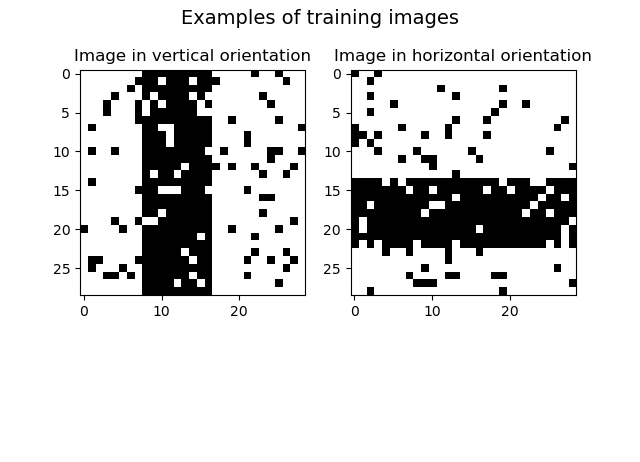
\includegraphics[width=\linewidth]{figures/horvert/horvertTrainingImages.png}
  \caption{Training images generated for experiment 2. One image of each possible orientation at a random position.}
  \label{fig:horvertImages}
\end{figure}

\begin{figure}
  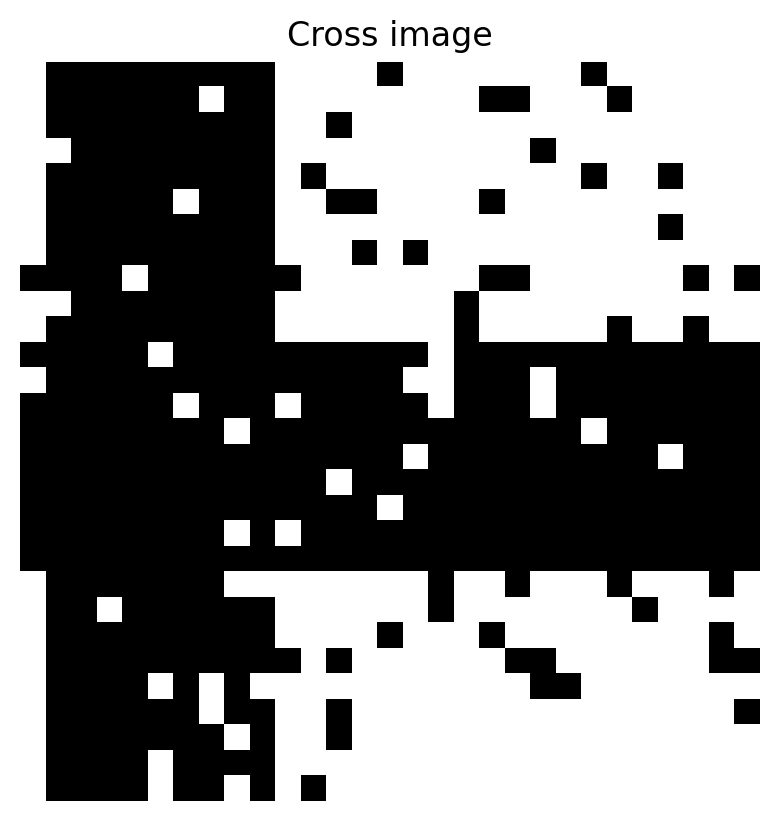
\includegraphics[width=0.6\linewidth]{figures/horvert/horvertTrainingCrossImage.png}
  \caption{Generated cross image which can represent either horizontal or vertical orientation.}
  \label{fig:horvertTrainingCrossImage}
\end{figure}


\paragraph{Network architecture}

This experiment used a expanded version of the network used in experiment 1. An additional layer of prior neurons $z_1,z_2$ was added. Whenever an image was oriented vertically $z_1$ was active and $z_2$ was inactive. For horizontal orientations $z_2$ was active and $z_1$ was inactive. Prior neurons in an active state had a firing frequency of 50 Hz and fired with 0 Hz when inactive.

\paragraph{Neuron model}
The input and output neurons functioned the same way as in the previous experiment. The prior neurons fire according to a poisson process with their firing rate. Each prior neuron $Z_l$ is connected to every output neuron $Y_k$ and thus has weights $w_{kl}$ that were learned by the network. 

\paragraph{Parameters}
As the amount of input neurons and the average number of black pixels in an input image stayed roughly the same in this experiment, the same parameters $c=  20$ and $\lambda = 10^{-3}$ could be used.

%% TODO START
%% this block was copied to Theoretical Background, cut this accordingly
%% Zfactor does not exist, remove!!!
 However as there are only two prior neurons, a way to amplify their produced signals was needed, otherwise their impact on the membrane potential of the output neurons would not be distinctive enough. So the EPSPs $z_l(t)$ were multiplied by the factor $Z_{factor}$. This factor was determined via grid search. The additional prior layer resulted in an expanded version of the membrane potential $u_k(t)$

\begin{equation}
\label{eqn:ukHorvert}
u_k(t) = \sum_{i=1}^n w_{ki} \cdot x_i(t) + \sum_{j=1}^n w_{kj} \cdot Z_{factor} \cdot z_j(t).
\end{equation}

%% TODO END

\subsection{Results} 

The following values for $Z_{factor} $ were tried with $c = 20$ and $\lambda = 10^{-3}$:
\begin{itemize}
  \item $Z_{factor} = 3$
  \item $Z_{factor} = 5$
  \item $Z_{factor} = 7$  
  \item $Z_{factor} = 10$ 
  \item $Z_{factor} = 20$
\end{itemize}

For $Z_{factor} = 10$ and $20$ the prior neurons impacted the learning progress negatively and let single prior neurons respond to too much area. An example of this can be seen in Figure \ref{fig:horvert_c20_3_Zfactor20_horizontalLines}

\begin{figure}
  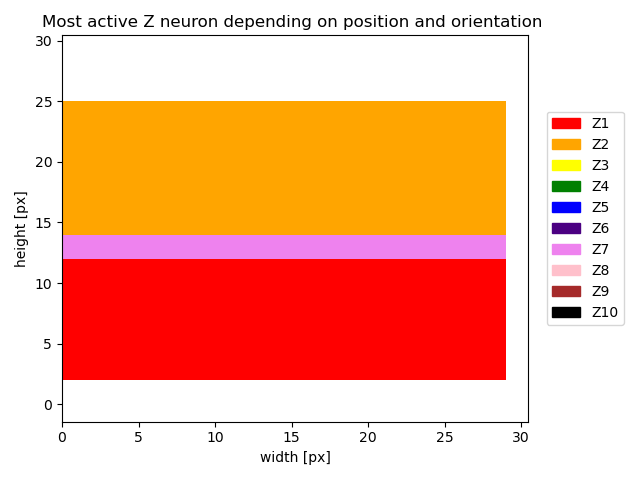
\includegraphics[width=\linewidth]{figures/horvert/horvert_c20_3_Zfactor20_horizontalLines.png}
  \caption{Most active output neuron for horizontal orientation and position on the y-axis of the training image during the training process. $c = 20, \lambda = 10^{-3}, Z_{factor} = 20$}
  \label{fig:horvert_c20_3_Zfactor20_horizontalLines}
\end{figure}


The best results were achieved with $Z_{factor} = 5$. When looking at the training progress in Figure \ref{fig:horvert_c20_3_Zfactor5_averageZ} it can be seen that the training accuracy is higher compared to experiment 1. This is due to the added a-priori information and the fact that less of each bar in an image is overlapping with multiple areas of output neurons. The network activity at the end of the training process can be seen in Figure \ref{fig:horvertLastSpikes}. In Figures \ref{fig:horvert_c20_3_Zfactor5_horizontalLines} and \ref{fig:horvert_c20_3_Zfactor5_verticalLines} the most active output neuron of the trained network is plotted for horizontal bars in every position and in the second plot for vertical bars in every position. Every one of the ten output neurons responds primarily to one coherent area in one orientation. The values of the learned prior weights $w_{kl}$ were plotted in Figures \ref{fig:wkl1} and \ref{fig:wkl2}. In these figures, in combination with Figures \ref{fig:horvert_c20_3_Zfactor5_horizontalLines} and \ref{fig:horvert_c20_3_Zfactor5_verticalLines}, can be seen that each prior neuron specialized on one orientation.

\begin{figure}
  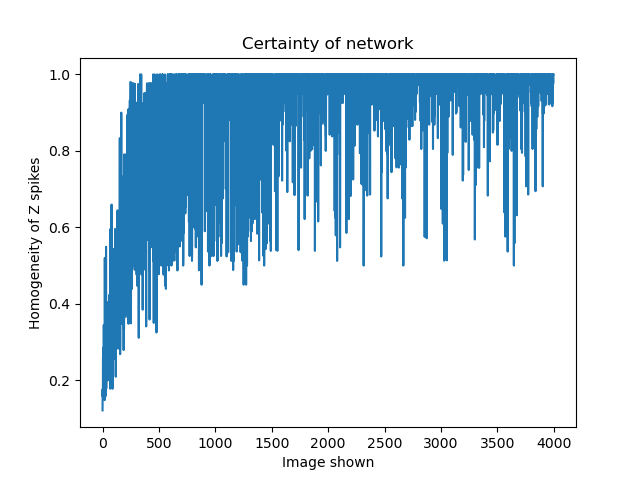
\includegraphics[width=\linewidth]{figures/horvert/horvert_c20_3_Zfactor5_averageZ.png}
  \caption{Proportion (accuracy) of most active output neuron  to activity of all other output neurons during the presentation duration of each training image. $c = 20, \lambda = 10^{-3}, Z_{factor} = 5$}
  \label{fig:horvert_c20_3_Zfactor5_averageZ}
\end{figure}

\begin{figure}
  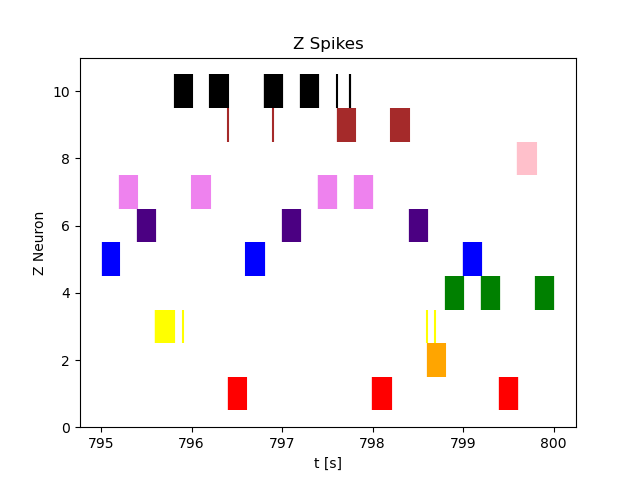
\includegraphics[width=\linewidth]{figures/horvert/horvert_c20_3_Zfactor5_1000LastZSpikes.png}
  \caption{Last 1000 output neuron spikes, $c = 20, \lambda = 10^{-3}$, $Z_{factor} = 5$}
  \label{fig:horvertLastSpikes}
\end{figure}

\begin{figure}
  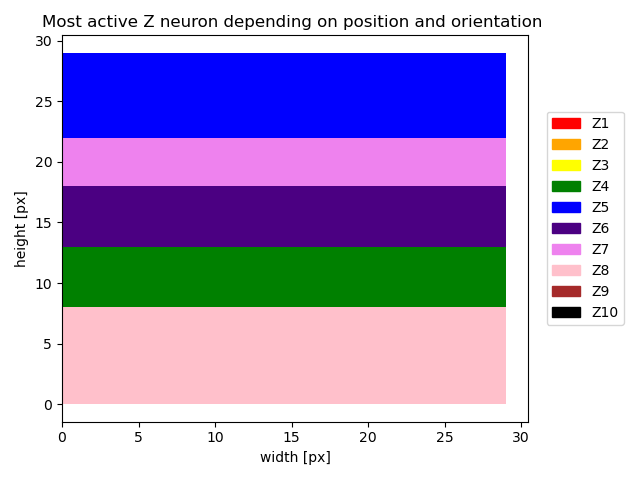
\includegraphics[width=\linewidth]{figures/horvert/horvert_c20_3_Zfactor5_horizontalLines.png}
  \caption{Most active output neuron for images of horizontal orientation and position on the x-axis of during the validation process. $c = 20, \lambda = 10^{-3}, Z_{factor} = 5$}
  \label{fig:horvert_c20_3_Zfactor5_horizontalLines}
\end{figure}

\begin{figure}
  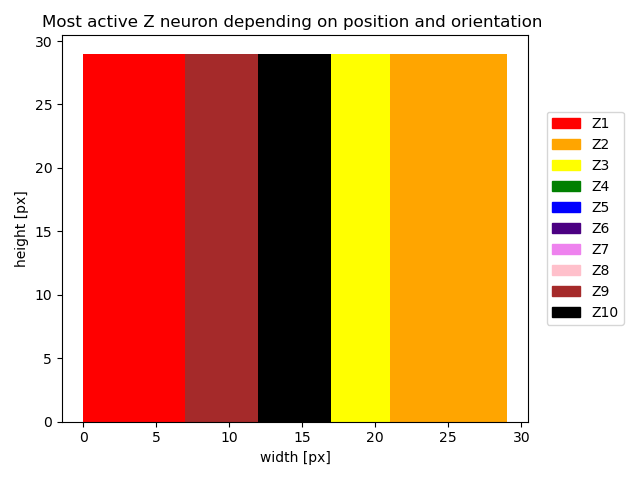
\includegraphics[width=\linewidth]{figures/horvert/horvert_c20_3_Zfactor5_verticalLines.png}
  \caption{Most active output neuron for images of vertical orientation and position on the x-axis of during the validation process. $c = 20, \lambda = 10^{-3}, Z_{factor} = 5$}
  \label{fig:horvert_c20_3_Zfactor5_verticalLines}
\end{figure}

\begin{figure}
  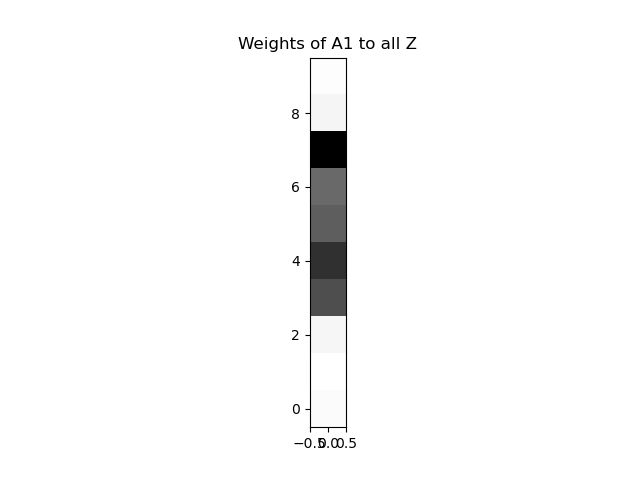
\includegraphics[width=\linewidth]{figures/horvert/horvert_c20_3_Zfactor5_priorWeight1.png}
  \caption{Values of $w_k1$, darker color means higher value. $c = 20, \lambda = 10^{-3}, Z_{factor} = 5$}
  \label{fig:wkl1}
\end{figure}

\begin{figure}
  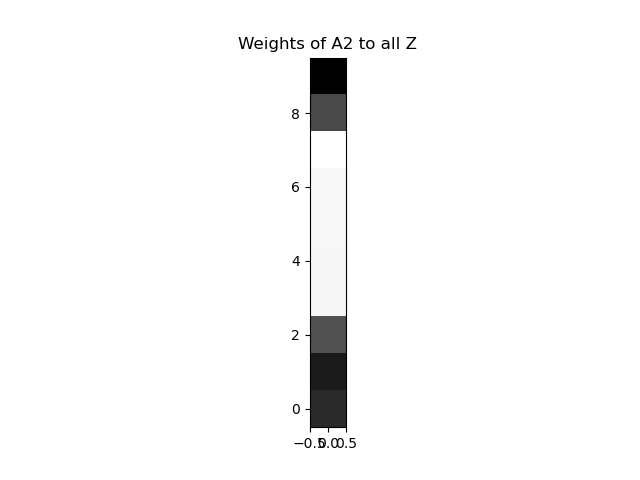
\includegraphics[width=\linewidth]{figures/horvert/horvert_c20_3_Zfactor5_priorWeight2.png}
  \caption{Values of $w_k2$, darker color means higher value. $c = 20, \lambda = 10^{-3}, Z_{factor} = 5$}
  \label{fig:wkl2}
\end{figure}

During the validation of all possible horizontal bar images the output spike activity was recorded and how many distinct output neurons were spiking during each image presentation period. For the parts where the 7 pixels high bar in the image did not overlap the areas of two output neurons only one output neuron was active. Only in the border areas there were two output neurons active. This can be seen in Figures \ref{fig:horvert_c20_3_Zfactor5_horizontalDistinctZ} and \ref{fig:horvert_c20_3_Zfactor5_horizontalZSpikes}. Compared to experiment 1 the activity is more homogeneous as each bar can only be in at most the area of four output neurons, when two of these areas are reinforced by the prior neurons.

\begin{figure}
  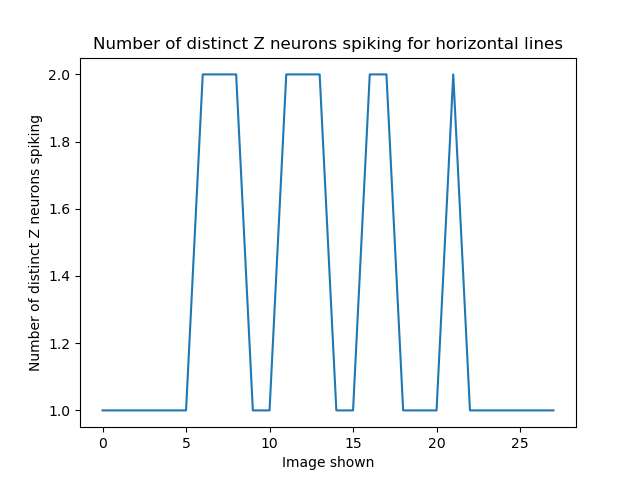
\includegraphics[width=\linewidth]{figures/horvert/horvert_c20_3_Zfactor5_horizontalDistinctZ.png}
  \caption{Distinct output neurons spiking during the presentation of all possible horizontal oriented validation images, $c = 20, \lambda = 10^{-3}$, $Z_{factor} = 5$}
  \label{fig:horvert_c20_3_Zfactor5_horizontalDistinctZ}
\end{figure}
\begin{figure}
  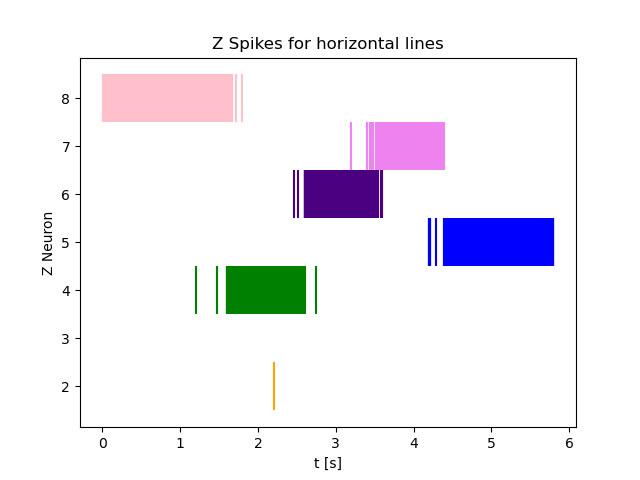
\includegraphics[width=\linewidth]{figures/horvert/horvert_c20_3_Zfactor5_horizontalZSpikes.png}
  \caption{Output neuron spikes during the presentation of all possible horizontal oriented validation images, $c = 20, \lambda = 10^{-3}$, $Z_{factor} = 5$}
  \label{fig:horvert_c20_3_Zfactor5_horizontalZSpikes}
\end{figure}


To show the impact of the prior neurons an image with two bars on it forming a cross (Figure \ref{fig:horvertValidationCross}) was generated and $z_2$ was set active indicating that the orientation is supposed to be horizontal. This resulted in the spiking pattern seen in Figure \ref{fig:horvert_c20_3_Zfactor5_crossZSpikes}. In it $Y_1$ is more active than $Y_9$ due to the influence of the prior neuron $Z_2$.

\begin{figure}
  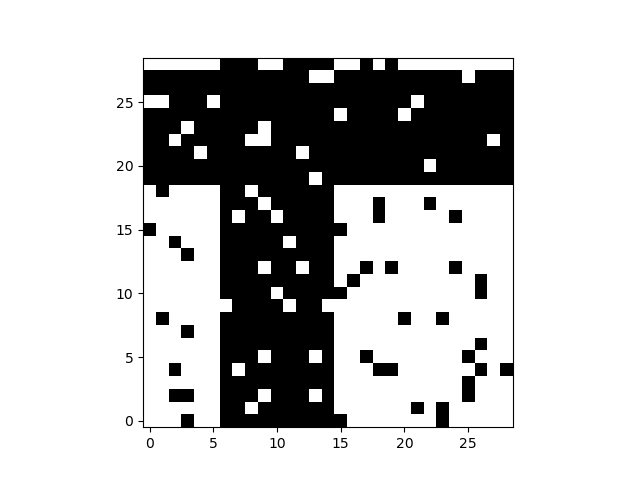
\includegraphics[width=\linewidth]{figures/horvert/horvert_c20_3_Zfactor5_validationCross.png}
  \caption{Generated validation cross image, with orientation defined as horizontal. $c = 20, \lambda = 10^{-3}, Z_{factor} = 5$}
  \label{fig:horvertValidationCross}
\end{figure}

\begin{figure}
  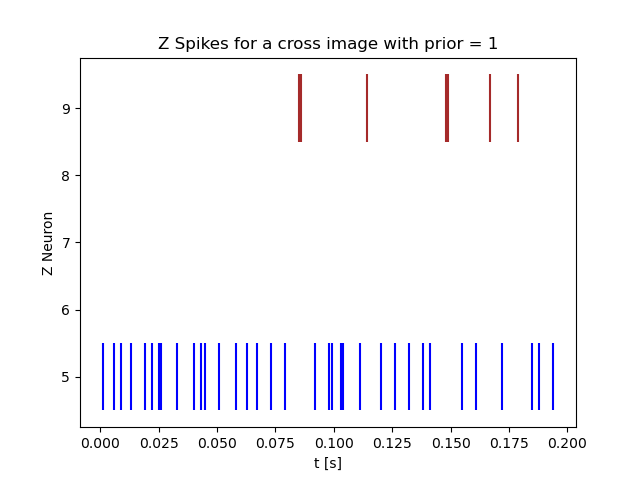
\includegraphics[width=\linewidth]{figures/horvert/horvert_c20_3_Zfactor5_crossZSpikes.png}
  \caption{Output spikes during the presentation of the validation cross image. $c = 20, \lambda = 10^{-3}, Z_{factor} = 5$}
  \label{fig:horvert_c20_3_Zfactor5_crossZSpikes}
\end{figure}

\fi